\documentclass[journal]{IEEEtran}
\usepackage{fontspec}
\setmainfont{texgyretermes}[Extension=.otf,UprightFont=*-regular,BoldFont=*-bold,
  ItalicFont=*-italic,BoldItalicFont=*-bolditalic]
\usepackage{unicode-math}
\setmathfont{texgyretermes-math.otf}
\usepackage{graphicx}
\usepackage{array}
\usepackage{booktabs}
\usepackage{cite}
\usepackage{url}
\usepackage{siunitx}
\sisetup{detect-all,per-mode=symbol}

\begin{document}

\title{Parked Loads: Protocol-Safe Wait-Until-Written\\Reads for Multi-Host CXL Memory}

\author{Romyull~Islam
\thanks{Manuscript draft, October 2026. R.~Islam is with Kennesaw State University, Kennesaw, GA,
USA (e-mail: mislam22@students.kennesaw.edu).}}% department to be added

\markboth{IEEE Computer Architecture Letters (draft)}{Islam: Parked Loads for Multi-Host CXL Memory}

\maketitle

\begin{abstract}
Hosts that share CXL memory have no cross-host hardware coherence unless the device implements
back-invalidation, so the systems built on it synchronize by flushing and polling or, like Tigon,
confine synchronization to a hardware-coherent region capped at 200\,MB, and
every poll is a device access that other tenants of the memory pool pay for. A CXL device could
instead hold a read of an unwritten line until another host's write lands, an idea as old as HEP's full/empty bits, but it must
do so without breaking the protocol: request credits are finite, hosts
fail independently, and a read that outlives the Root Port's completion timeout fails and can
isolate the port. We give five rules under which a device parks a CXL.mem read safely, and show
with the TLC model checker that together they rule out Root Port timeouts, unwritten data and
blocked writers. In gem5, with x86 programs on up to 36 hosts, parked waiters wait with 1.4 to 1.5
reads per message instead of 39 when messages arrive every \SI{20}{\micro\second}, and with 256 waiters the pool's tenants keep over 99\% of
their bandwidth instead of 77 to 79\%. A parked flag is 1.02 to 1.18$\times$ faster than uncached
flag polling and 1.07 to 1.51$\times$ faster than flush polling for handoffs and RPCs, and a parked cache-line fill is 1.25 to 1.28$\times$ faster than the
best software scheme we test for one-line messages.
\end{abstract}

\begin{IEEEkeywords}
CXL, memory pooling, synchronization, full/empty bits, multi-host shared memory
\end{IEEEkeywords}

\section{Introduction}
CXL 2.0 pools a memory device among up to 16 hosts, each region dedicated to one host; CXL 3.0 adds
shared memory that two or more hosts load and store, and back-invalidation (BI) for hardware coherence.
Shared memory exposed as HDM-H supports only software coherence between hosts~\cite{cxl3}, and
Tigon caps its hardware-coherent region at 200\,MB~\cite{tigon}. Cross-host communication therefore
runs on software protocols: a producer writes a message and a flag, and the consumer flushes its
cached copy and re-reads the flag until it changes. MPI and RPC over CXL poll message
queues~\cite{cmpi,hydrarpc}, a GPU collective library polls a per-chunk doorbell in the
pool~\cite{cccl}, and TraCT, which hands KV cache from prefill to decode servers through CXL memory
for LLM serving~\cite{tract}, polls and flushes lock state per node; acquiring an
uncontended lock takes about \SI{20}{\micro\second} with 2 nodes and \SI{100}{\micro\second} with 16
in its naive design~\cite{tract_thesis}. On an FPGA multi-headed device a flushed access takes
\SI{2.2}{\micro\second}, 2.8$\times$ a cached one~\cite{cmpi}.

\begin{figure}[t]
\centering
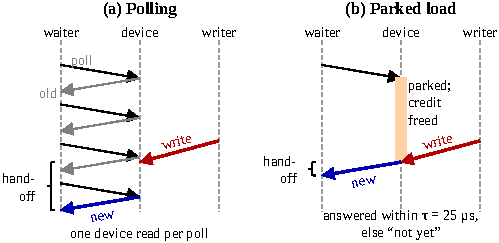
\includegraphics[width=\columnwidth]{fig_idea.pdf}
\caption{A waiter on one host and a writer on another share a CXL device. (a) Polling: each poll is
a device read; the waiter sees the write at its next poll. (b) Parked load: the device holds the read
without holding a request credit and answers it when the write lands, or answers ``not yet'' within
$\tau$, below the Root Port completion timeout.}
\label{fig:idea}
\end{figure}

Polling has two costs (Fig.~\ref{fig:idea}a). The waiter learns of the write only at its next poll,
and each poll is a device access, so waiting threads consume bandwidth that other tenants of a
shared pool need: in our runs, 256 polling waiters cut four streaming tenants from 44.8 to 34.3 to
\SI{35.5}{\giga\byte\per\second}. The device is the only place that sees both the waiting read and the releasing
write, so it can answer the read when the write lands (Fig.~\ref{fig:idea}b). Holding a read in
memory until it can be satisfied dates to HEP and I-structures (Section~\ref{sec:prior}); we do not claim the waiting
primitive. We claim that it can be made safe on CXL.mem, where the waiter and the writer are
independent hosts behind a switch or a multi-headed device, request credits are finite, a read must
not outlive a completion timeout whose expiry fails it and can isolate the port, the protocol has
no response that means \emph{not yet}, and hosts fail separately. This letter contributes:
\begin{itemize}
\item five rules under which a CXL device parks a CXL.mem read, and the host rules that make
parking work with caches and prefetchers (Section~\ref{sec:design});
\item a TLA+ model~\cite{tla} with which the TLC model checker~\cite{tlc} shows the rules sufficient
for 2 and 3 consumers, 2 credits and a 2-entry table, and four of them individually necessary (Section~\ref{sec:verify});
\item an implementation of the device in gem5~\cite{gem5}, run with x86 programs on up to 36 hosts,
that measures handoff latency and the fabric bandwidth polling waiters take from other tenants
(Section~\ref{sec:eval}).
\end{itemize}

\section{Parked Loads}
\label{sec:design}
\textbf{Synchronization region.} The fabric manager marks an HDM range as a synchronization region.
The device keeps one full/empty bit per 64\,B line, in SRAM (\SI{128}{\kibi\byte}
covers a \SI{64}{\mebi\byte} region) or in device-private spare bits, not in the host-visible HDM-H metadata.
A write to a line stores the data, sets it \emph{full} and answers the reads parked on it. A second
address window makes a read \emph{consuming} (it also sets the line empty, for single-consumer
queues) and makes a write set the line empty. A read of an empty line moves from the request queue into a
parked table keyed by line address; Table~\ref{tab:rules} lists the five rules that keep this safe.

\begin{table}[t]
\centering
\caption{The five rules, the CXL property behind each, and what the TLC model checker finds when
the rule is removed (shortest counterexample in states).}
\label{tab:rules}
\scriptsize\setlength{\tabcolsep}{3pt}
\begin{tabular}{@{}>{\raggedright}p{2.35cm}>{\raggedright}p{2.75cm}>{\raggedright\arraybackslash}p{3.2cm}@{}}
\toprule
Rule & CXL basis & Without it \\
\midrule
\textbf{R1} Parking frees the request credit & a credit returns when the receiver frees the message
buffer~\cite{cxl3} & the producer's ordinary read waits $\tau$ (8) \\
\textbf{R2} The releasing write is never blocked & writes use the RwD channel; with BI, RwD must pass
Req~\cite{cxl3} & nothing on its own, R1 implies it; without R1 too, the write waits $\tau$ (11) \\
\textbf{R3} Every parked read is answered within $\tau$ & CXL.mem timeout of \SI{50}{\micro\second} to
\SI{10}{\milli\second} by default, settable to 50 to \SI{100}{\micro\second}~\cite{cxl32} & a read outlives the Root Port timeout (9) \\
\textbf{R4} That answer says \emph{not yet} & CXL 3.0 DRS has only MemData and MemData-NXM~\cite{cxl3} &
a consumer accepts unwritten data (8) \\
\textbf{R5} A read for ownership is never parked & HDM-H requests carry no snoop type~\cite{cxl32} & a
write-back writer waits $\tau$ (17) \\
\bottomrule
\end{tabular}
\end{table}

\textbf{The rules.} \emph{R1:} parking moves the read out of the request queue, so other requests
keep flowing; responses never block, because the requester preallocates its NDR and DRS
buffers~\cite{cxl3}. \emph{R2:} with R1 no parked read occupies the request queue, so no write
waits behind one; apart from same-address cases CXL orders neither message classes nor
different addresses, so answering a parked read after later requests is legal, and a device already holds a
read to a line with an outstanding back-invalidate snoop~\cite{cxl3}. \emph{R3:} when software
enables timeout and isolation, an expired read gets a synthesized error response and the port is
isolated~\cite{cxl32}, so the device answers every parked read within $\tau=\SI{25}{\micro\second}$, half the
\SI{50}{\micro\second} minimum timeout.
\emph{R4:} the device returns the line's current contents, and software sees an unchanged sequence
number and re-issues, so a long wait costs one access per $\tau$; a reserved metadata value (HDM-H
metadata, where the device stores it, is host defined~\cite{cxl32}) or a new DRS opcode can mark the
reply explicitly. A full table answers at once, which degrades to polling. \emph{R5:} a store that
misses in a write-back mapping first reads the line for ownership, and an HDM-H device cannot tell
that read from a shared one, so writers update sync lines with stores that do not read the line:
uncached stores, or MOVDIR64B, which neither fetches nor caches the 64\,B line~\cite{intelsdm}. A
host that marks its ownership reads in the metadata bits lets the device answer them at once.

\textbf{Host side.} A waiter parks with an \emph{uncached} load of a flag, which never issues
speculatively, or with a \emph{cacheable} line fill: it flushes its copy and loads the line, and the
wake-up delivers the whole 64\,B line, so a one-line message arrives with the wake-up. A speculative
or prefetched fill only holds a miss buffer until the wake-up or $\tau$. Cacheable parked reads are
non-consuming, so a prefetch cannot take a message; the waiter empties the line afterwards with a
store to the consuming window, off the critical path. A writer that uses write-allocating stores, as
in our parked line fill runs, could wait in the miss buffer of its own parked prefetch; placing each
sync line on its own 4\,KiB page prevents this for the L2 streamer and adjacent-line prefetchers,
which stay within a page, but not for the next-page prefetcher in Intel's optimization manual~\cite{intelopt}. The
non-allocating stores of R5 remove the case. A parked load stalls its thread, and delays an
interrupt to that core, by at most $\tau$.

\textbf{Failures, fairness and cost.} When a host fails or its logical device is reset, the device
drops that host's entries (a design rule we did not model); waiters of a failed producer see
\emph{not yet} every $\tau$ and decide after how many to give up. Wake-up is FIFO per line. An entry holds the
line address, the requester's port and tag and a timer, at most 16\,B; 4,096 entries take
\SI{64}{\kibi\byte}.

\textbf{Prior art.}\label{sec:prior} HEP and the Tera MTA retried accesses to
empty locations~\cite{tera}, and I-structures queued deferred reads at the
location~\cite{istructures}. IBM's conditional load waits in a memory-controller table until a store
or a timer within the processor's load deadline~\cite{ibmclt}; Microsoft's conditional wait can be
deferred at the memory controller with a timeout~\cite{msftcond}; reads of unavailable data in the
Synchronization State Buffer fail rather than wait~\cite{ssb}; QOSB (later QOLB) keeps a hardware queue of
lock waiters among caches~\cite{qolb}; Lustig and Martonosi stall GPU reads
of empty locations at the memory controller until a CPU write and leave timeouts to future
work~\cite{lustig}; Callback reads block in a dedicated directory at the last-level cache until a
write~\cite{callback}; LRSCwait's Mwait holds a request at a memory bank of a 256-core cluster until
the watched location is written~\cite{lrscwait}; RISC-V's WRS.STO stalls a core until a store to its
reservation set or a short timeout~\cite{zawrs}; and IBM's queue control holds requests to locked
addresses with a time to live and signals an expired one with a memory-error interrupt rather than
a reply~\cite{ibmqueue}. These work inside one machine, where no fabric credit rule applies; IBM's
conditional-load bound is a processor load deadline, not a Root Port timeout. In CXL, Intel's patents queue atomic
operations per host in a device~\cite{intelq} and queue keyed lock requests~\cite{intellock}, a
dual-headed device offers test-and-set and compare-and-swap in CXL.io registers~\cite{amdshare}, and
Micron's device defers requests to cache ways busy with another operation~\cite{micron}; outside
CXL, Intel forwards MONITOR/MWAIT through network controllers to a remote node~\cite{intelmwait}.
None holds a plain read until another host writes the data, and none bounds a held read by the
Root Port completion timeout; Intel's device times out back-invalidate responses only to detect a
failed host~\cite{intelq}.

\section{Verification}
\label{sec:verify}
The TLA+ model has consumer hosts that wait on one sync line, a producer that first reads an
ordinary line and then writes the sync line (through a write-back mapping in one variant, so with a
read for ownership), request credits, the RwD channel, a bounded parked table, the device timeout
and the Root Port timeout. The producer may wait arbitrarily long and may fail; time advances only
when no host or device step that cannot wait is enabled, and credit arbitration is fair. TLC checks
four invariants (no read outlives the Root Port timeout; a consumer never accepts unwritten data; the
producer's ordinary read and its releasing write never wait as long as $\tau$) and one liveness
property (if the producer lives, every consumer gets the data), for 2 and 3 consumers sharing 2
credits and a 2-entry table, with a device timeout of 2 and a Root Port timeout of 4 ticks. With all
five rules every property holds (up to 8,572 states). Removing R1, R3, R4 or R5 breaks the property
it protects (Table~\ref{tab:rules}); R2 alone is redundant once R1 holds, because a parked read then
holds no credit.

\section{Evaluation}
\label{sec:eval}
\textbf{Setup.} We add the device to gem5 v25.1~\cite{gem5} (CXL-ClusterSim couples gem5 with SST for
pooled memory~\cite{cxlclustersim}) as a memory object: SimpleMemory timing
(\SI{100}{\nano\second} access, a \SI{64}{\gibi\byte\per\second} port, at least one 64\,B line per
access), full/empty bits, two address windows, a parked table and the timeout. Each host is its own
gem5 system with out-of-order x86 cores (gem5's TimingSimpleCPU for barriers, waiters and
posters), 32\,KiB L1s, a 1\,MiB L2 with a stride prefetcher and its own coherence domain; hosts reach
the device through a link of \SI{32}{\giga\byte\per\second} with a one-way flight delay of 63, 78 or
\SI{238}{\nano\second}, meeting at a
\SI{64}{\giga\byte\per\second} shared crossbar. The idle uncached round trip is
\SI{124.5}{\nano\second} plus twice the flight delay, which we set to model a
\SI{250}{\nano\second} expander, a \SI{280}{\nano\second} multi-headed device and a
\SI{600}{\nano\second} switch, within the 230--270, 260--300 and 490--\SI{600}{\nano\second}
measured by Octopus~\cite{octopus}. Static x86 programs run on every host and time handoffs with
the simulated clock. Protocols: \emph{flush} poll (clflushopt, fence, load of a flag),
\emph{uncached} poll, \emph{line} poll (re-read the payload lines until all carry the new sequence
number, the fastest software scheme we test), \emph{parked flag} (uncached) and \emph{parked line
fill}. In the parked line fill, writers use write-back stores, and the device recognizes their
ownership reads directly (gem5's needsWritable flag), standing in for the marking of R5; the parked
flag is written with uncached stores. gem5 charges a flush only its cache work, while the cMPI
measurements imply \SI{1.4}{\micro\second} (a flushed access of \SI{2.2}{\micro\second}
against a cached one of \SI{0.79}{\micro\second})~\cite{cmpi}, so gem5 undercharges every flush poll. As
a cross-check of the polling baseline, our discrete-event model (in the artifact) gives
\SI{890}{\nano\second} for uncached flag polling of a 64\,B message on the expander and gem5
\SI{944}{\nano\second}. We count \emph{waiting reads}: the reads of a flag or line until the
waiter sees the message; every protocol except the parked line fill then reads the payload once.

\begin{table}[t]
\centering
\caption{Latency in gem5 (\si{\micro\second}): one-way handoff with the consumer waiting, zero-work RPC with
256\,B messages, and a 16-host barrier round. Best per column in bold; line polling has no
barrier variant.}
\label{tab:lat}
\scriptsize\setlength{\tabcolsep}{3.5pt}
\begin{tabular}{@{}lrrrrr@{}}
\toprule
 & 64\,B & 64\,B & 1\,KiB & RPC & barrier \\
protocol & expander & switch & switch & switch & switch \\
\midrule
flush poll & 1.20 & 2.80 & 3.35 & 5.73 & 12.53 \\
uncached poll & 0.94 & 2.18 & 2.77 & 4.59 & \textbf{11.01} \\
line poll & 0.66 & 1.52 & \textbf{2.01} & \textbf{3.32} & n/a \\
parked flag & 0.80 & 1.85 & 2.44 & 3.94 & 11.06 \\
parked line fill & \textbf{0.52} & \textbf{1.22} & 3.03 & 5.75 & 20.83 \\
\bottomrule
\end{tabular}
\end{table}

\textbf{Latency.} For one-line messages a parked line fill is fastest on every device: 517, 577 and
\SI{1216}{\nano\second} on the expander, multi-headed device and switch, 1.25 to 1.28$\times$ faster
than line polling, 1.8$\times$ than uncached and 2.3$\times$ than flush polling
(Table~\ref{tab:lat}). Longer messages need a doorbell and a payload read, and the write-back
doorbell store first reads the line for ownership, so line polling is fastest there and the parked
line fill is 3 to 11\% slower than uncached polling. The parked flag is 1.03 to 1.18$\times$ faster
than uncached and 1.1 to 1.5$\times$ faster than flush polling for every message size, and 1.02 to
1.17$\times$ and 1.07 to 1.45$\times$ for RPCs. Line polling remains the fastest RPC scheme, and the
parked line fill pays the ownership read there (1.04 to 1.25$\times$ slower than uncached polling). Barrier
rounds with a parked flag are within 1.4\% of uncached polling, because the master's sequential scan
of arrival flags, one round trip each, dominates; a parked line fill is 1.5 to 1.9$\times$ slower
there, because each arrival and release store first reads the line for ownership. MOVDIR64B, which
gem5 does not model, would remove that read.

\begin{figure}[t]
\centering
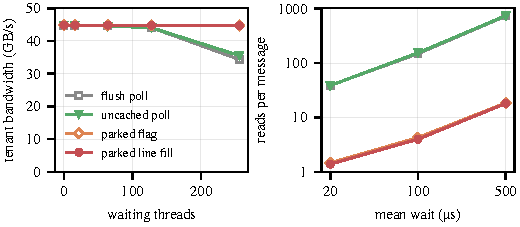
\includegraphics[width=\columnwidth]{fig_contention.pdf}
\caption{(a) Bandwidth of four streaming tenant hosts on the switched device next to waiting
threads (messages every \SI{20}{\micro\second} on average). (b) Waiting reads per message for 64
waiters as the mean wait grows past $\tau$. Parked flag and parked line fill overlap, as do flush and
uncached polling.}
\label{fig:cont}
\end{figure}

\textbf{Shared-device contention.} Four tenant hosts stream reads at \SI{44.8}{\giga\byte\per\second}
alone, next to waiter hosts (16 waiters each), each fed by its own poster host (36 hosts in all
at 256 waiters). Up to 128 polling
waiters cost the tenants under 2\%; with 256, every waiter issuing a device read per round trip,
39 per message, adds up to \SI{32}{\giga\byte\per\second} of polls (39 reads of 64\,B per waiter
and message, one message per \SI{20}{\micro\second} on average plus posting time), the device saturates, and the tenants drop to 34.3
(flush) and \SI{35.5}{\giga\byte\per\second} (uncached) (Fig.~\ref{fig:cont}a). Parked waiters issue
1.4 to 1.5 waiting reads per message, the tenants keep 44.6 to \SI{44.7}{\giga\byte\per\second}, and handoff
stays at 1.25 (line fill) and \SI{1.93}{\micro\second} (flag) against 2.25 and
\SI{2.88}{\micro\second} for polling. With 64 waiters and a mean wait of \SI{500}{\micro\second}, 20
times $\tau$, a parked read times out and re-parks every \SI{25}{\micro\second}: 18 waiting reads per
message against 740 to 750 for polling (Fig.~\ref{fig:cont}b), with handoff latency within 4\% of the
\SI{20}{\micro\second} case. A table with fewer entries than waiters degrades toward polling:
with 128 or 32 entries for 256 waiters, overflowing reads are answered at once and retried (13 to
32 reads per message), and the tenants keep 43.8 to 44.0 and 38.0 to
\SI{39.1}{\giga\byte\per\second}, still more than with polling.

\textbf{Limitations.} gem5 runs the programs in syscall-emulation mode, models the switch as a
crossbar, and models neither back-invalidate coherence nor MOVDIR64B; hardware flushes cost more
than gem5 charges, which favors polling. Each point is one deterministic run, with up to \SI{2}{\micro\second} of random delay per message:
28 handoffs or RPCs, 18 barrier rounds, and 4 to 15 messages per waiter in the contention runs. The
TLA+ model has one sync line and one producer, and only the producer fails; host failure in the
device is not modeled.

\textbf{What deployment needs.} No change to CXL.mem messages: R1 to R3 are device behavior within
the existing rules, R4 answers with an ordinary data response, and R5 uses existing stores. Software
needs one sync line per 4\,KiB page, a sequence number per message and a give-up policy for failed
producers; the device adds a parked-table lookup on every write to the region.

\section{Conclusion}
A multi-host CXL device can hold a read until another host writes the line without breaking
CXL.mem's credit, ordering and timeout rules, if it follows five rules; four of them are each
needed. Parking stops waiters from taking a pooled device's bandwidth from its tenants. The open
steps are an
FPGA prototype and a \emph{not yet} reply defined in the CXL specification.

\textbf{Artifact.} The gem5 model, programs, TLA+ model and results are at
\url{https://github.com/Romyull-Islam/CXL-Research} (folder 3-parked-loads).

\bibliographystyle{IEEEtran}
\bibliography{p3}

\end{document}
